\documentclass{article}
\usepackage{tikz}

\begin{document}

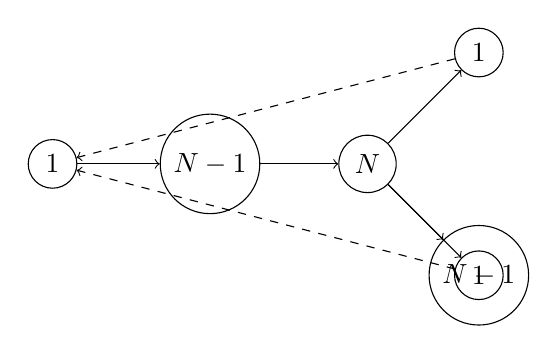
\begin{tikzpicture}[node distance=2cm]
    \node[circle,draw] (1) {$1$};
    \node[circle,draw] (N-1) [right of=1] {$N-1$};
    \node[circle,draw] (N) [right of=N-1] {$N$};
    \node[circle,draw] (N-1') [below right of=N] {$N-1$};
    \node[circle,draw] (1') [above right of=N] {$1$};
    \node[circle,draw] (1'') [below right of=N] {$1$};

    \draw[->] (1) -- node {} (N-1);
    \draw[->] (N-1) -- node {} (N);
    \draw[->] (N) -- node {} (N-1');
    \draw[->] (N) -- node {} (1');
    \draw[->] (N) -- node {} (1'');

    \draw[dashed,->] (1') -- node {} (1);
    \draw[dashed,->] (1'') -- node {} (1);
\end{tikzpicture}

\end{document}